\chapter{Conclusioni}
\label{chap:Conclusioni}

Il modello sviluppato in questo studio è stato progettato per automatizzare la segmentazione di
immagini di femori fetali \cite{abstract1} \cite{abstract2}. L'utilizzo del modello consente di
automatizzare un compito che altrimenti richiederebbe tempo e impegno da parte di un professionista,
liberando risorse per altre attività.

Specificamente, il modello è stato impiegato per automatizzare l'estrazione dei pixel del femore di
un feto nelle settimane 35-37 di gestazione. I pixel estratti sono stati analizzati per determinare
la luminosità, che nelle ecografie è correlata alla \textbf{densità minerale ossea} (\textbf{BMD})
del femore fetale, e per studiarne la correlazione con il peso di nascita.

Una correlazione debole è stata rilevata tra la luminosità e il peso alla nascita, come illustrato
nella Figura \ref{fig:correlazione tra luminosità e peso alla nascita}.

\begin{figure}[!ht]
    \centering
    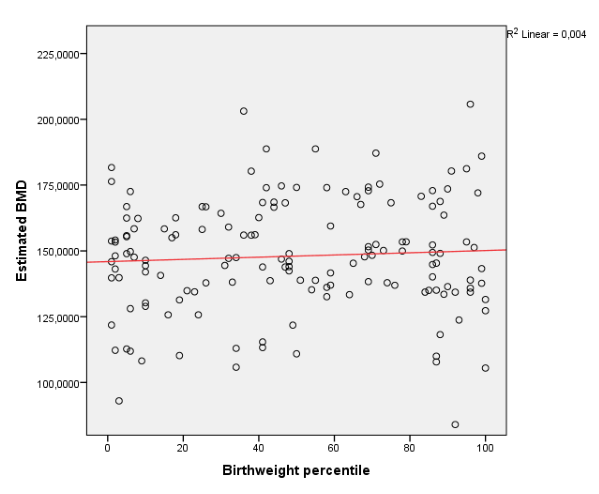
\includegraphics[width=0.6\columnwidth]{Immagini/correlation_weight_abstract.png}
    \caption{Correlazione tra luminosità e peso alla nascita}
    \label{fig:correlazione tra luminosità e peso alla nascita}
\end{figure}

La rete neurale ha dimostrato di essere efficace nel riconoscere i pixel contenenti informazioni
sull'area del femore. Inoltre, i risultati prodotti dalla rete suggeriscono la possibilità di
utilizzare questo approccio per ulteriori analisi.
